\documentclass{myclass}

\usepackage{multicol}
\usepackage{wrapfig}
\usepackage[utf8]{inputenc}
\usepackage{mathtools}
\usepackage{esint}
\usepackage{amsmath}
\usepackage{amssymb}
\usepackage{amsmath,amsfonts,amssymb,amsthm,epsfig,epstopdf,titling,url,array}
\usepackage{hyperref}
\usepackage{eso-pic}
\usepackage{array}

\newcommand{\incfig}[1]{%
  \def\svgwidth{0.9\columnwidth}
  \import{./figures/}{#1.pdf_tex}
}

\newcommand{\incimg}[1]{%
    \includegraphics[width=0.9\columnwidth]{images/#1}
}

\title{Termodinámica}

\begin{document}
\maketitle
\tableofcontents
\newpage

\section{Fundamentales}

\subsection{Termómetro}

\subsection{Varaibles intensivas y extensivas}
Las variables \textit{intensivas} son aquellas independientes de la masa ($T, p, \rho$).
Las \textit{extensivas} son las proporcionales a la masa ($V, U, S$) \\
\\
Podemos hacer intensivas variables extensivas (variable específica) dividiendo por la masa ($v = \frac{V}{m}, \rho = \frac{m}{V} = \frac{1}{v}$). \\
Podemos hacer intensivas variables extensivas (variable molar específica) dividiendo por los moles.

\subsection{Dilatación y compresibilidad}
Si queremos buscar una función de estado podemos operar diferencialmente sabiendo que por la regla de la cadena:
$$
dV = (\frac{\partial V}{\partial P})_Tdp + (\frac{\partial V}{\partial T})_PdT
$$
Definiendo las siguientes variables tenemos:
$$
\begin{cases}
\alpha = \frac{1}{V}(\frac{\partial V}{\partial T})_P & \text{coef. \textit{dilatación isobárica}} \\
\chi = -\frac{1}{V}(\frac{\partial V}{\partial P})_T & \text{coef. \textit{compresibilidad isotérmica}}
\end{cases}
\implies \boxed{\frac{dV}{V} = \alpha dT - \chi dP}
$$
\\
Supongamos que tenemos el caso concreto donde la presión no varía pero sí la temperatura.
Entonces la ecuación de estado diferencial se simplifica
$$
\frac{dV}{V} = \alpha dT \implies \int_{V_0}^V\frac{dV}{V} = \int_{T_0}^T\alpha dT \implies V=V_0(1+\alpha\Delta T)
$$
para $\Delta T$ pequeños \footnote{\label{fn1} Hemos usado la aproximación del supuesto $\alpha$ constante en el pequeño intervalo y la serie de Taylor $e^{\alpha\Delta T} \approx 1+\alpha \Delta T$}.
\\
También podemos hacer esto con la superficie y la longitud de los materiales
\begin{center}
    \begin{tabular}{c c c c}
    \textbf{Constante} & \textbf{Tipo} & \textbf{Ecuación} & \textbf{Relación} \\
    $\alpha$ & volúmica & $V=V_0(1+\alpha \Delta T)$ & $\alpha = 3\lambda$ \\ 
    $\sigma$ & superficial & $S=S_0(1+\sigma \Delta T)$ & $\sigma = 2\lambda$ \\ 
    $\lambda$ & lineal & $L=L_0(1+\lambda \Delta T)$  &
\end{tabular}
\end{center}
En general si hay cambios de presión y temperatura
$$
V = V_0(1+\alpha\Delta T - \chi \Delta P)
$$

\subsection{Ecuación de estado}
En un sistema termodinámico podemos encontrar la \textit{función de estado} si este sistema se encuentra en \textit{equilibrio termodinámico}. Esto es, cuando las variables termodinámicas no varían en el tiempo. La ecuación de estado será de la forma:
$$
\boxed{f(P, v, T) = 0} 
$$
\textbf{Antecedentes}
\begin{itemize}
    \item \textit{Ley de Boyle.} Isotermas $PV=cte$
    \item \textit{Ley de Gay-Loussac.} Isobáricas $V/T=cte$
    \item Isocóricas $P/T=cte$
\end{itemize}
Experimentalmente se observa que para los gases ideales se cumple $\boxed{Pv=RT}$ ($v$ molar específica). \\
\\
No obstante no se ajusta a los gases reales. 
%\begin{wrapfigure}{r}{0.45\textwidth}
%    \begin{center}
%    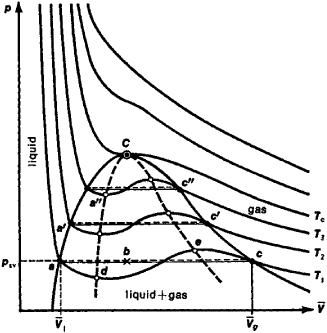
\includegraphics[width=0.4\textwidth]{images/van-der-waals.png}
%  \end{center}
%\end{wrapfigure}
\begin{multicols}{2}[\columnsep2em]
\noindent
\textbf{Van del Waals} $ \ \
\boxed{(P+\frac{a}{v^2})(v-b) = RT}$ \\
$
\\
\implies Pv^3 - (Pb + RT)v^2 + av - ab = 0
$\\
Para $a, b$ constantes dependientes de los gases. \\
Para calcular el punto crítico observamos \\ $\left(\frac{\partial P}{\partial v}\right)_T = 0, \quad \left(\frac{\partial^2 P}{\partial v^2}\right)_T = 0$ \\
Calculando tenemos \\
$P_c = \frac{a}{27b^2}, \quad v_c = 3b, \quad T_c = \frac{8a}{27Rb} \ \ \ \ \ \ \ \ \ \ \ \ \ $ 
\columnbreak
    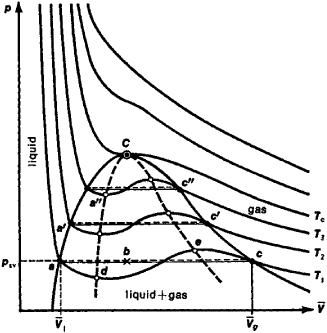
\includegraphics[scale=0.4]{images/van-der-waals.png}
\end{multicols}
\noindent
\textbf{Dieterici} \ \
$
\boxed{P = \frac{1}{v-b}RTe^{-\frac{a}{RTv}}}
$\\
\\
La temperatura de Boyle es $T_{Boyle} = \frac{a}{bR}$ \\
\\
\textbf{Coeficientes de Virial} \ \
$
\boxed{Pv = RT(1+ \frac{B(T)}{v} + \frac{C(T)}{v^2} + \ldots)}
$
\\ \\
Se realiza una correccion con un desarrollo en serie de potencias. \\
La temperatura de Boyle es la que cumple $B(T_{Boyle})=0$
\subsection{Diagrama de fase}
Si representamos el diagrama Pv tenemos una campana en cuyo interior coexisten líquido y vapor. La isoterma dentro de la campana se realiza a $P$ constante. 
\newline

\begin{multicols}{2}[\columnsep2em]
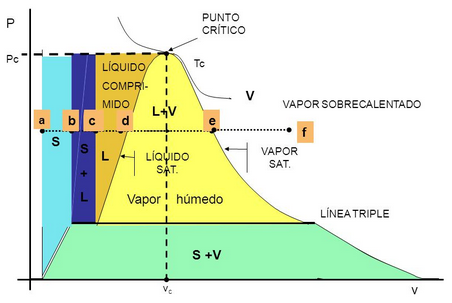
\includegraphics[scale=0.5]{images/Pv_fases.png}
\columnbreak
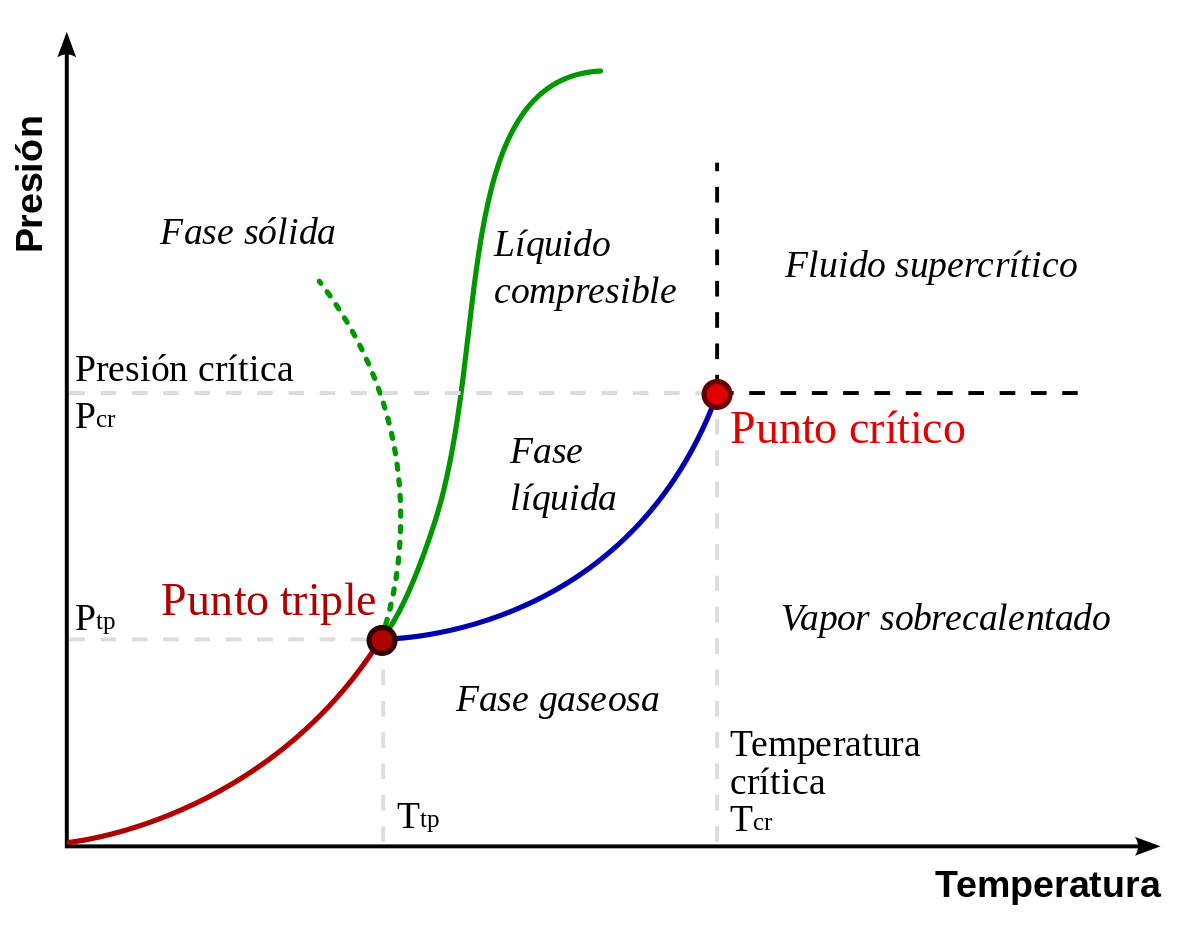
\includegraphics[scale=0.12]{images/PT-fase.png}
\end{multicols}
\noindent
Existe un Punto triple donde coexisten los tres estados y un punto crítico por encima del cual no hay transición de fase.

\subsection{Tipos de procesos}
\begin{itemize}
    \item \textit{Isotérmico:} $T$ constante
    \item \textit{Isobárico:} $P$ constante
    \item \textit{Isocórico:} $V$ constante
    \item \textit{Adiabático:} Aislado (no intercambio de calor)
    \item \textit{Reversible:} se puede invertir su sentido
\end{itemize}



\subsection{Humedad}
Definiremos tres términos:
\begin{itemize}
    \item \textbf{Humedad Absoluta} $H_a = \frac{m_v}{V}$
    \item \textbf{Humedad Relativa} $H_r=\frac{m_v}{m_s} = \frac{P_v}{P_s}$
    \item \textbf{Punto de rocío} $P_v=P_s$
\end{itemize}
Al hacer problemas debemos tener en cuenta que $P_a + P_v = P_t$ y que el aire cumple $P_aV_a = P'_aV'_a$

\section{Primer principio de la termodinámica}
\subsection{Trabajo}
Podemos escribir el trabajo como $\boxed{d'W = P_edV} \implies W = \int_{V_1}^{V_2}P_edV$ \\
Si el proceso es reversible $P = P_e$. \\
Ponemos $d'W$ en lugar de $dW$ porque es una diferencial inexacta al depender el trabajo del camino en el que se integra. Por esta razón $W$ no es una propiedad del sistema. \\
\\
A continuación el trabajo en diferentes sistemas
\begin{itemize}
    \item \textbf{Isócora} $W = 0$
    \item \textbf{Isobárica} $W = P(V_2-V_1)$
    \item \textbf{Isotérmica} $W = nRT\ln{\frac{V_2}{V_1}}$
    \item \textbf{Isotérmica en sólidos} $W = -V_0\chi\int_{P_1}^{P_2}PdP = -\frac{V_0\chi}{2}(P_2^2-P_1^2)$
    \item \textbf{Isobárica en sólidos} $W = P\alpha V_0\int_{T_1}^{T_2}dT = V_0\alpha P (T_2-T_1)$
\end{itemize}
\subsection{Calor específico}
Definiciones
\begin{itemize}
    \item \textbf{Capacidad calorífica} $C=\frac{d'Q}{dT} \implies \begin{cases}
    C_p \text{ a presión constante} \\
    C_V \text{ a volumen constante}
    \end{cases}$
    \item \textbf{Calor específica} $c=\frac{C}{m}$
    \item \textbf{Calor latente} $L$ calor necesario para cambiar de estado.
\end{itemize}

Definimos la variable $\boxed{dU := d'Q - d'w}$, que si que es variable de estado, donde $Q<0$ si lo produce el sistema (exotérmico) y $Q>0$ si es suministrado al sistema (endotérmico). \\
\\
Definimos también la Entalpía $\boxed{H:=U+PV}$ \\
\\
\textbf{Primer principio de la termodinámica:} El trabajo adiabático $\boxed{W^{ad}_{a\to b} = -\Delta u}$ es el mismo en en todos los procesos adiabáticos.
Equivalentemente 




\section{Calor}
Tres tipos de Propagación del calor
\begin{itemize}
    \item \textbf{Conducción:} Contacto directo, sin movimiento de materia.
    \item \textbf{Convención:} Movimiento de materia.
     \item \textbf{Radiación:} Propagación de ondas electromagnéticas en el vacío, sin medio material.
\end{itemize}
\subsection{Conducción}
Definimos la variable $q$ como densidad superficial de flujo de calor (dirigida hacia temperaturas más bajas):
$$
q = \frac{d^2Q}{dtds} = \frac{d\dot{Q}}{ds} \implies d\dot{Q} = \Bar{q}\cdot d\Bar{s}
$$
La ley de Fourier nos dice $\boxed{\Bar{q} = -\lambda \cdot \Bar{\nabla}T}$ siendo $\lambda$ la conductividad térmica. Por otro lado tenemos que $\Bar{\nabla}\cdot \Bar{q} = -c_e\rho\frac{dT}{dt}$. \\
De estas dos ecuaciones la \textit{Ecuación de Fourier o conducción del calor}:
$$
\boxed{\nabla^2T=\frac{1}{\alpha}\frac{dT}{dt}}, \qquad \alpha = \frac{\lambda}{c_e\rho}
$$
Siendo $\alpha$ la difusividad térmica del medio

\section{Aplicaciones del Primer Principio}
\subsection{Relación de Mayer generalizada}
\[
  \left( \frac{\partial U}{\partial T} \right)_v = C_v , \quad \left( \frac{\partial H}{\partial T} \right)_p=C_p \implies C_p=C_v + \left( \left( \frac{\partial U}{\partial V} \right)_T + p  \right)V\alpha 
\] 
\subsection{Experimento Joule-Gay Lussac}
Expansión de un gas hacia otro recipiente inicialmente en vacío. Se cumple:
\[
\Delta U = 0, \quad \Delta T=0, \left( \frac{\partial U}{\partial V}_T \right) =0
\] 

\subsection{Experimento de Joule-Kelvin}
El proceso se trata de una expansión adiabática irreversible a través de una membrana. En un proceso de Joule-Kelvin se cumple:
\[
dH=0 
\] 
\subsection{Calores molares en un gas ideal}
Sabemos por la relación de Mayer que $C_p = C_V + nR$
 \begin{center}
\begin{tabular}{|c|c|c|}
\hline
 & $c_V$ & $c_P$ \\
\hline 
  Gases monoatómicos & $\quad \frac{3}{2}R\quad$ & $\quad \frac{5}{2}R\quad$ \\
  \hline
  Gases diatómicos & $\quad\frac{5}{2}R\quad$ & $\quad\frac{7}{2}R\quad$ \\
  \hline

\end{tabular}
\end{center}

\subsection{Transformación adiabática}
En una transformación adiabática reversible tenemos:
\[
dU = -pdV, \quad pv^\gamma=cte
\] 

\section{Máquinas térmicas y Segundo Principio}
\subsection{Máquinas térmicas}
\begin{multicols}{2}[\columnsep2em]
Una \textbf{Máquina térmica} es un dispositivo de funcionamiento cíclico que tiene como objetivo producir trabajo mecánico gracias al calor absorbido y cedido por una sustancia termodinámica activa. \\
\columnbreak
\incimg{MaquinaTermica.png}
\end{multicols}
\begin{multicols}{2}[\columnsep2em]
  Existen dos tipos de máquinas a las que suministramos trabajo $W$
\begin{itemize}
  \item \textbf{Máquina Frigorífica:} absorbe la mayor cantidad posible de calor
  \item \textbf{Bomba Térmica:} cede la máxima cantidad posible de calor 
\end{itemize}
\columnbreak
\incimg{MaquinaFrigorifica.png}
\end{multicols}
Podemos definir la eficiencia de una máquina frigorífica y de una bomba térmica como
\[
\mathcal{E}_{MF} = \frac{Q_2}{|W|} = \frac{T_2}{|T_1- T_2|}, \qquad \mathcal{E}_{BT} = \frac{Q_1}{W} = \frac{T_1}{T_1- T_2}
\]
Donde las segundas igualdades se cumplen si y solo si el proceso es reversible

\subsection{Segundo principio}
Dos enunciados equivalentes del segundo principio:
\begin{itemize}
    \item \textbf{Kelvin-Planck:} $\nexists$ máquina térmica con $\eta = 1$
    \item \textbf{Clausius:} $\nexists$ $\begin{cases}
    \text{bomba térmica} \\
    \text{máquina frigorífica}
    \end{cases}$ con $\mathcal{E}= \infty$
\end{itemize}
\subsection{Ciclo de Carnot}
\begin{multicols}{2}[\columnsep2em]
    \incimg{CicloCarnot.png}
\columnbreak                                                                                                   
   \begin{itemize}
     \item $1\to 2$ expansión isotérmico
	 \item  $2\to 3$ expansión adiabática
	 \item  $3\to 4$ compresión isotérmica
   	 \item $4\to 1$ compresión adiabática
   \end{itemize}
   \[
  \eta = 1 + \frac{Q_2}{Q_1} = 1- \frac{T_2}{T_1} \\
   \] 
   \textbf{Teorema de Carnot}\\
   Máquina $\begin{cases}
     \text{Reversible } \implies \eta_R = \eta_C \implies \frac{Q_1}{T_1} + \frac{Q_2}{T_2} = 0 \\
     \text{Irreversible } \implies \eta_I < \eta_C \implies \frac{Q_1}{T_1} + \frac{Q_2}{T_2} < 0 
   \end{cases}$

\end{multicols}

\section{Entropía y segundo principio}
\subsection{Definición}
Definimos la función de estado entropía $S$, que en forma diferencial se expresa como $dS = \frac{\delta Q_{rev}}{T}$, con $Q_{rev}$ el calor reversible intercambiado. \\
\\
Como es función de estado el teorema de Clausius se puede enunciar:
\[
\begin{cases}
  \displaystyle\oint_C S = \oint_C \frac{\delta Q_{rev}}{T} = 0 \iff \text{ C reversible} \\
  \displaystyle\oint_C S = \oint_C \frac{\delta Q_{rev}}{T} <  0 \iff \text{ C irreversible}
\end{cases}
\] 
La segunda ley de la termodinámica es equivalente a su formulación con entropía $\boxed{\Delta S_{univ}\ge 0}$ \\
\\
La energía que se pierde en los procesos irreversibles se llama energía no reutilizable, y se puede obtener con la fórmula $E_{no\ util} = T_0\Delta S_{univ}$, donde $T_0$ es la mínima temperatura involucrada en el proceso.

\subsection{Cálculo de la entropía}
Podemos calcular la variación de entropía mediante las tres expresiones equivalentes (up to constant):
\begin{align*}
  S &= nc_p\ln T - nR\ln p + S_0 \\  
  S &= nc_v\ln T - nR\ln V + S_0 \\  
  S &= nc_p\ln V - nc_vR\ln p + S_0 \\  
\end{align*}
Al ser $S$ extensiva $\displaystyle S_T = \sum_{i=1}^{N} S_i$ \\
\\
\begin{minipage}{0.7\textwidth}
Si lo que tenemos son compartimentos con diferentes gases y se liberan estos gases la entropía variará como:
$$\displaystyle\Delta S_g=-R \sum_{i=1}^{N} n_i\ln\chi_i$$
\end{minipage}
\begin{minipage}{0.25\textwidth}
    \incimg{MezclaGases.png}
\end{minipage}

\section{Potenciales termodinámicos}
Disponemos de 4 funciones de estado con dimensiones de energía. Las vemos en una tabla
\begin{center}
\begin{tabular}{|c|c|c|c|}
  \hline
  Definición & Variables & Forma diferencial & Derivadas \\
  \hline
  Energía interna & $U(S, V)$  & $dU = TdS - pdV$ & $\displaystyle T = \left( \frac{\partial U}{\partial S} \right)_V, \quad -p = \left( \frac{\partial U}{\partial V} \right)_S  $ \\
  \hline
  Entalpía & $H(S, V) = U + pV$  & $dH = TdS - Vdp$ & $\displaystyle T = \left( \frac{\partial H}{\partial S} \right)_p, \quad V = \left( \frac{\partial H}{\partial p} \right)_S  $ \\
  \hline
  Función de Helmholtz & $F(T, V)=U-TS$  & $dF = -SdT - pdV$ & $ \displaystyle  -S = \left( \frac{\partial F}{\partial T} \right)_V, \quad \boxed{-p = \left( \frac{\partial F}{\partial V} \right)_T}  $ \\
  \hline
  Función de Gibbs & $G(T, p) = H-TS$  & $dG = -SdT + Vdp$ & $\displaystyle -S = \left( \frac{\partial G}{\partial T} \right)_p, \quad \boxed{V = \left( \frac{\partial G}{\partial p} \right)_T } $ \\
  \hline
  
\end{tabular}
\end{center}
Además por el teorema de Schwartz se cumple (Relaciones de Maxwell):
\[
  \left( \frac{\partial T}{\partial V} \right)_S = -\left( \frac{\partial p}{\partial S} \right)_V , \qquad \left( \frac{\partial T}{\partial p} \right)_S = \left( \frac{\partial U}{\partial S} \right)_p, \qquad \left( \frac{\partial S}{\partial V} \right)_T = \left( \frac{\partial p}{\partial T} \right)_V, \qquad \left( \frac{\partial S}{\partial p} \right)_T = -\left( \frac{\partial V}{\partial T } \right)_p
\] 
Con las dos ecuaciones encuadradas podemos deducir la ecuación de estado si sabemos la función de Helmholtz o la de Gibbs. 
\subsection{Significado físico de los potenciales}
Cada incremento de potencial tiene un significado físico:
\begin{itemize}
  \item $\Delta U = -W_{adiabatico}$ 
  \item $\Delta H=Q_{isobarico}$ 
  \item $\Delta F = -W_{reversible}$ 
  \item $\Delta G = -W^*_{reversible}$
\end{itemize}

\subsection{Ecuaciones $TdS$}


\section{Transiciones de fase}















\end{document}

